
% !TeX spellcheck = en

\chapter{Database Change Scenarios}
This section shows how to handle the predefined scenarios for the given change management tool. This includes following scenarios: 

\begin{itemize}
	\item Rename an attribute.
	\item Add an attribute and set the value as a constant.
	\item Delete an attribute.
	\item Change an attribute type and add an SQL script to fill it from existing values.
	\item Rename a table and change a related view which uses this table.
\end{itemize}


\section{Flyway Scenarios}

\subsection{Usage \& minimal Example}

\marginpar{CLI and commands}%
\textbf{Migrate}\\
To create a first migration, add a database change as sql file into the sql directory (see \autoref{fig:flyway_sql_scripts}).
In our minimal example, the file \texttt{V1\_\_create\_db.sql} looks like the following:

\begin{lstlisting}[language=SQL, caption=Create a database]
	CREATE TABLE weather (
	city            varchar(80),
	temp_lo         int,           -- low temperature
	temp_hi         int,           -- high temperature
	prcp            real,          -- precipitation
	date            date
	);
\end{lstlisting}

To apply the first migration, run: \texttt{flyway migrate}.
If the migration is successful, you will see the output below:
\begin{lstlisting}[caption=Flyway first migration success]
	(base) marco@MacBook-Pro-von-Marco flyway-9.6.0 % flyway migrate
	Flyway is up to date
	Flyway Community Edition 9.6.0 by Redgate
	See what's new here: https://flywaydb.org/documentation/learnmore/releaseNotes#9.6.0
	
	Database: jdbc:postgresql://localhost:5433/seminar (PostgreSQL 14.5)
	Successfully validated 1 migration (execution time 00:00.021s)
	Creating Schema History table "public"."flyway_schema_history" ...
	Current version of schema "public": << Empty Schema >>
	Migrating schema "public" to version "1 - create db"
	Successfully applied 1 migration to schema "public", now at version v1 (execution time 00:00.030s)
\end{lstlisting}

Now the table \textit{weather} has been created by flyway. There was also an additional metadata table (\textit{flyway\_schema\_history}) created with the first migration. This metadata table holds various information regarding the migration and their past.

If one want to update the database for example with data, just create a new script with the name e.g. \texttt{V2\_\_add\_data.sql} and run  \texttt{flyway migrate} again.

\begin{lstlisting}[language=SQL, caption=Create a database]
	INSERT INTO weather VALUES ('Zurich', 10, 17, 0.25, '2022-10-30');
	INSERT INTO weather VALUES ('Rapperswil', 8, 15, 0.25, '2022-10-30');
\end{lstlisting}

\begin{figure}[H]
	\centering
	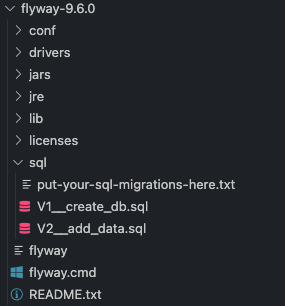
\includegraphics[width=0.4\textwidth]{./chapters/intro_flyway/images/flyway_v2_sql_migrations}
	\caption[Flyway SQL migrations - Source: Own illustration]{Flyway SQL migrations}
	\label{fig:flyway_sql_scripts}
\end{figure}





\subsection{Usage with Java API, Maven or Gradle}
\marginpar{JavaAPI}%
LOBs,

\marginpar{Maven or Gradle}%
Integration with maven or gradle.


\section{Liquibase Scenarios}



\newpage